\subsection{Lock exchange}

% NOTE equivalent vertical diffusivity due to spurious mixing appears to be about 5e-6 or so

The lock exchange test case (\cref{fig:lock-snapshot}) is a simple configuration that shows the creation of intermediate densities by spurious mixing. This is a replication of one of the test cases presented by \citet{ilicak12}. The test case takes place in a two-dimensional domain of 64km width and 20m depth. Only the highest resolution test cases are chosen, with horizontal and vertical grid spacings of $\Delta x = \SI{500}{\metre}$ and $\Delta z = \SI{1}{\metre}$, respectively. In this case, and the following cases, the explicit vertical diffusivity is set to zero, so that all mixing must be spurious. The lock exchange is defined by an initial temperature distribution comprised of one density class on each side of the domain,
%
\begin{equation}
  \Theta(x) = \begin{cases}
    \SI{5}{\celsius} & x < \SI{32}{\kilo\metre}\\
    \SI{30}{\celsius} & x \ge \SI{32}{\kilo\metre}.
  \end{cases}
\end{equation}

\begin{figure}
  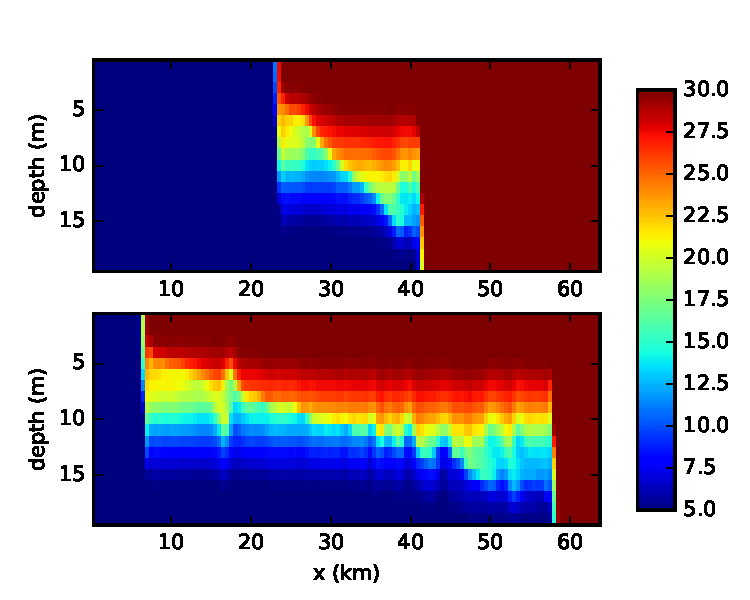
\includegraphics{{../plots/lock_exchange_snapshot_0.01}.pdf}
  \caption{\label{fig:lock-snapshot} Snapshots of lock exchange at 6 hours (top) and 17 hours (bottom) at $\nu_h = \SI{0.01}{\square\metre\per\second}$. Temperature (\si{\celsius}) is shown in colours. Spurious mixing at the front can be seen by the presence of intermediate temperatures.}
\end{figure}

This case is equivalent to two adjacent basins, each at constant temperature, with a dam between them that is removed at $t=0$. The warm water from the right basin flows from right-to-left above cold water, while conversely cold water from the left basin flows underneath the warm water from left-to-right. This is simply a gravity current, for which we have a theoretical prediction for the front velocity in a rectangular channel, given by
%
\begin{equation}
  u_f = \frac12 \sqrt{gH \Delta\rho / \rho_0},
\end{equation}
%
where $H$ is the domain depth and $\Delta\rho$ is the density difference across the front, normalised by a reference velocity. When calculating the grid Reynolds number, the theoretical front velocity is used instead of the actual mean velocity over the domain to match \citet{ilicak12}. All runs were carried out for 17 hours using a baroclinic timestep that satisfied CFL conditions across the range of horizontal viscosities (\SIlist{0.01;0.1;1;10;100;200}{\square\metre\per\second}).

\begin{figure}
  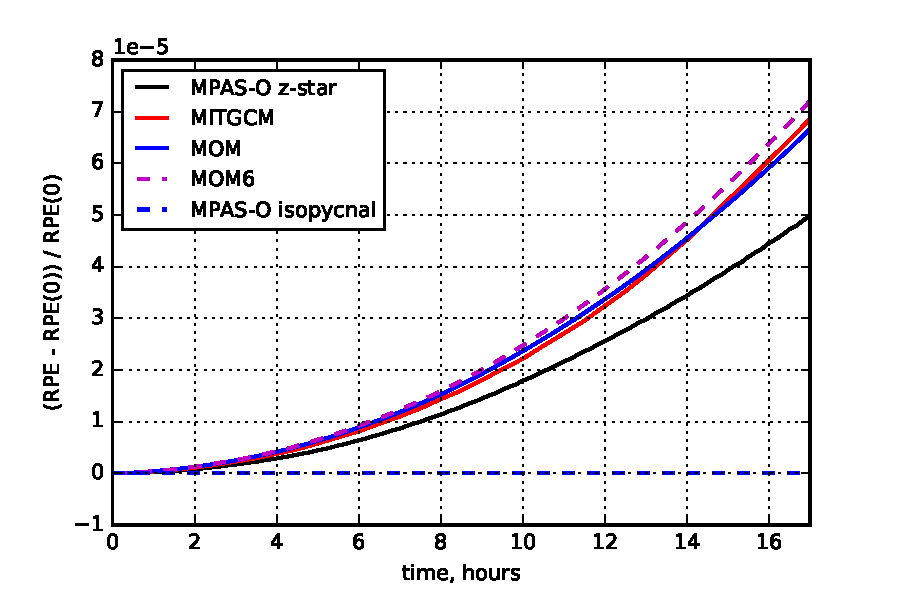
\includegraphics{../plots/lock_exchange_rpe_norm.pdf}
  \caption{\label{fig:lock-rpenorm} Normalised RPE evolution for $\nu_h = \SI{0.01}{\square\metre\per\second}$. MITGCM and MOM results come from \citet{ilicak12}, while MPAS-O results come from \citet{petersen15}. MOM6 exhibits a larger increase in RPE due to spurious mixing.}
\end{figure}

\begin{figure}
  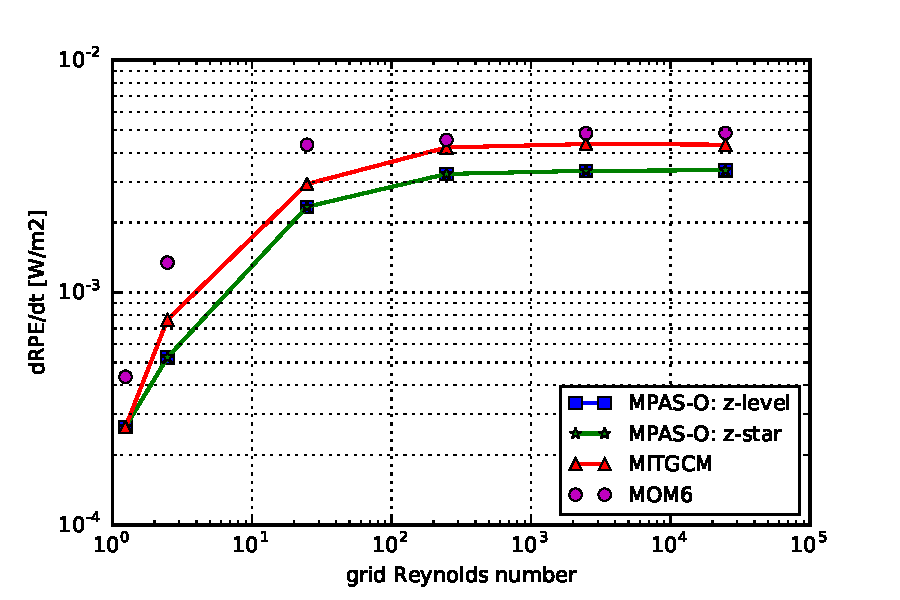
\includegraphics{../plots/lock_exchange_drpe.pdf}
  \caption{\label{fig:lock-drpe} Instantaneous rate of RPE change at 17h. MPAS-O and MITGCM results come from \citet{petersen15} and \citet{ilicak12} respectively. MOM6 exhibits a higher rate of change, and therefore spurious mixing, particularly in the unsaturated regime where $\mathrm{Re}_\Delta < O(10)$}
\end{figure}

The time series of normalised RPE in \cref{fig:lock-rpenorm} shows MOM6 having a similar shape to MITGCM and MOM. However, the actual values of the normalised RPE are greater in MOM6, suggesting that more spurious mixing is occurring in MOM6. 

Above a grid Reynolds number of 10, MOM6 performs slightly worse than the other models shown in \cref{fig:lock-drpe}. At this point, the models are running above the threshold for saturation of spurious mixing. However, in the regime where spurious mixing isn't saturated, MOM6 exhibits a higher rate of RPE change. This result suggests that spurious mixing in MOM6 is due to tracer advection, as viscosity in the unsaturated regime is sufficient to damp grid-scale noise in the velocity field.

% NOTE look at wavenumber spectrum of velocity field

\subsubsection{Advection order}
One aspect of model configuration that may significantly affect spurious mixing is the order of accuracy of the tracer advection scheme. A higher-order advection scheme purports to reduce the spurious mixing in advection, at the cost of runtime performance. Curiously, the two advection schemes in MOM6, PLM (piecewise linear) and the Huynh third-order piecewise parabolic scheme, PPM:H3 \citep{huynh97}, exhibit nearly identical spurious mixing. In order to preserve the pre-existing range of density classes by avoiding the creation of spurious minima or maxima, advection schemes may employ limiters. In MOM6, the limiting scheme reduces to a first-order upstream method. The minimal difference in spurious mixing despite an improved advection scheme suggests that advection may be dominated by a limiter at the front, where spurious mixing is most vigorous.

% NOTE can this be checked? where is the limiter active?

\subsubsection{Equivalent diffusivity}
% XXX incomplete section
% - maybe include figure?
By running the model with an explicit vertical diffusivity, we can compare the additional mixing introduced to the baseline spurious mixing when explicit diffusivity is disabled. In the lowest viscosity regime, the rate of change of RPE is approximately doubled with an explicit diffusivity $\kappa_D = \SI{e-5}{\square\metre\per\second}$, suggesting that the equivalent spurious diffusivity is on this order of magnitude.

\subsubsection{Spurious mixing orientation}
\begin{figure}
  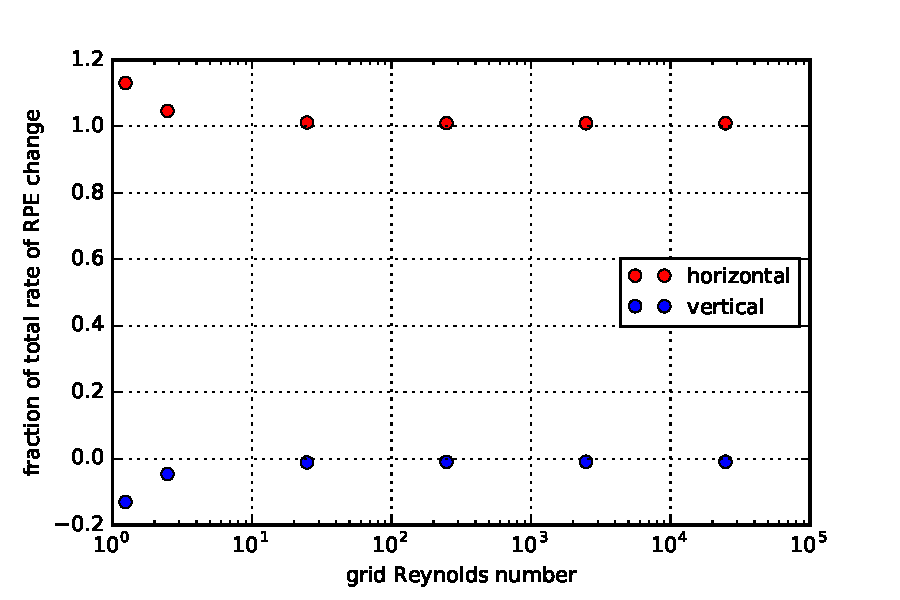
\includegraphics{../plots/lock_exchange_drpe_split.pdf}
  \caption{\label{fig:lock-rpesplit} Horizontal and vertical contributions to the instantaneous rate of RPE change at 17h}
\end{figure}

\Cref{fig:lock-rpesplit} shows that the mixing is predominantly due to horizontal processes. Indeed, for all of the experiments, the average RPE change due to regridding/remapping is actually negative. Physically, this means that regridding/remapping tends to slightly lower the centre of mass of the domain, counteracting some of the centre of mass increase due to mixing by the advection scheme. The magnitude of this compensation by regridding/remapping is negligible, so the spurious mixing is still set by the tracer advection scheme. Therefore, MOM6 exhibits slightly more spurious mixing than the other tested models, due primarily to the tracer advection scheme.
